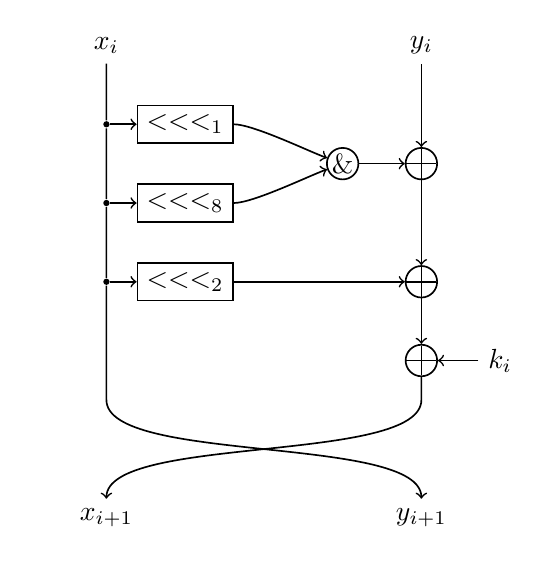
\begin{tikzpicture}
	[line width=0.6,trim left,
	box/.style = {
		draw
	},
	loosewire/.style = {
		looseness=0.5,
	},
	xor/.style = {
		draw, circle, inner sep=0cm, minimum size=0.4cm,
		append after command = {
			[shorten >=\pgflinewidth, shorten <=\pgflinewidth,]
			(\tikzlastnode.north) edge (\tikzlastnode.south)
			(\tikzlastnode.east) edge (\tikzlastnode.west)
		}
	},
	odot/.style = {
		draw, circle, inner sep=0cm, minimum size=0.4cm
	},
	dot/.style = {
		fill, circle, inner sep=0cm, minimum size=0.08cm
	},
	invisible/.style = {
		minimum size=0cm
	}]
	
	%Draw nodes
	\node at (1,7) (xin) {$x_i$};
	\node at (5,7) (yin) {$y_i$};
	\node[dot] at (1,6) (d1) {};
	\node[dot] at (1,5) (d2) {};
	\node[dot] at (1,4) (d3) {};
	\node[box] at (2,6) (S1) {$<<<_1$};
	\node[box] at (2,5) (S2) {$<<<_8$};
	\node[box] at (2,4) (S3) {$<<<_2$};
	\node[xor] at (5,5.5) (x1) {};
	\node[xor] at (5,4) (x2) {};
	\node[xor] at (5,3) (x3) {};
	\node[odot] at (4,5.5) (AND) {$\&$};
	\node at (6,3) (k) {$k_i$};
	\node at (1, 1) (xout) {$x_{i+1}$};
	\node at (5, 1) (yout) {$y_{i+1}$};
	\coordinate (cright) at (5, 2.5);
	\coordinate (cleft) at (1, 2.5);
	
	%Draw wires
	\draw[->] (d1) -- (S1);
	\draw[loosewire,->] (S1.east) to[out=0, in=160] (AND);
	\draw[->] (d2) -- (S2);
	\draw[loosewire,->] (S2.east) to[out=0, in=200] (AND);
	\draw[->] (AND) -- (x1);
	\draw[->] (d3) -- (S3);
	\draw[->] (S3.east) -- (x2);
	\draw[loosewire,->] (xin) -- (d1) -- (d2) -- (d3)
	-- (cleft) to[out=270, in=90] (yout.north);
	\draw[->] (yin) -- (x1);
	\draw[->] (x1) -- (x2);
	\draw[->] (x2) -- (x3);
	\draw[loosewire,->] (x3) -- (cright) to[out=270, in=90] (xout.north);
	\draw[->] (k.west) -- (x3);
\end{tikzpicture}%